\chapter{Discussion on the Performance Measurements}
\section{Discussion of test setup}
All our tests was run in a Lenovo Thinkpad T420 as seen on Figure \ref{fig:hardware}. The laptop was black and well equipped with both a coffe mug holder and an I5 processor running at 4983.98 bogomips, with 4GB of RAM. Each test was run 10 times to produce the statistics, although any variance in the test results might be caused by one or more kernels being used to browse facebook and other things at the same time.

\begin{figure}[H]
    \centering
    
\includegraphics[width=0.8\textwidth]{hardware.jpg}
    \label{fig:hardware}
    \caption{The physical hardware setup used for testing}
\end{figure}


\section{Performance plots}
Our graphs seen in Figure \ref{fig:throughput} and \ref{fig:latency}, these graphs has been generated on the data generated in our tests which can be seen in Appendix \ref{app:output}. It can be observed that the goodput in our setup shows the expected tendencies, especially on the local test where it is clearly visible how the goodput decreases when concurrency increases, as the overhead increases.

When we instead look at the latency we have a variance in our remote and local tests, where we can see that in both the tests we start off with a relatively high latency in the test with a single user, which is then decreased when we add additional concurrent requests. We can then see two expected trends, where the remote version increases in latency in relation the the increase in concurrency, while the local version does not due. This is most likely due to the giant overhead caused by using the TCP sockets and HTTP to communicate.

\begin{figure}[h!]
    \centering
    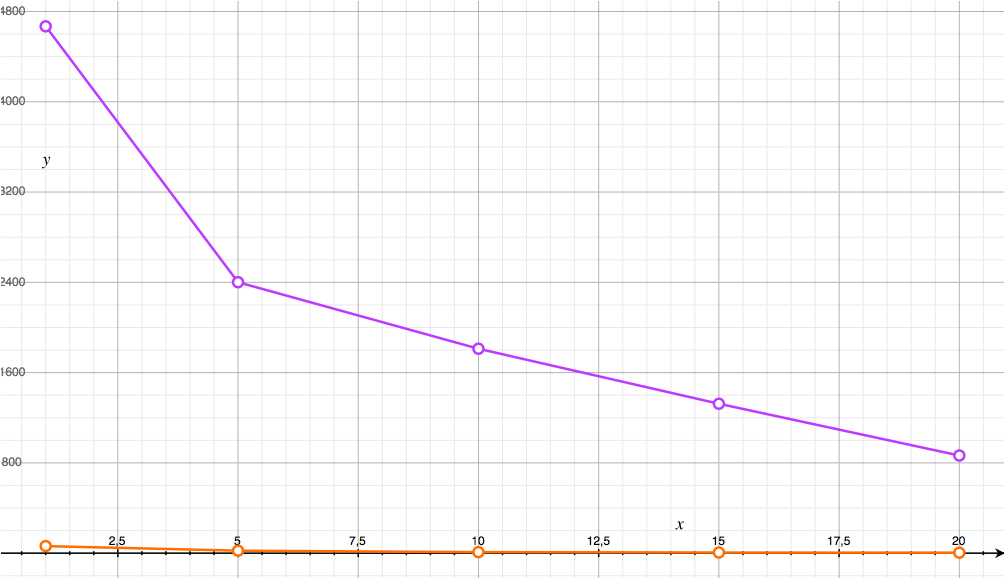
\includegraphics[width=0.8\textwidth]{graf1.jpg}
    \label{fig:throughput}
    \caption{Graph showing local vs remote goodput in our tests}
\end{figure}

\begin{figure}[h!]
    \centering
    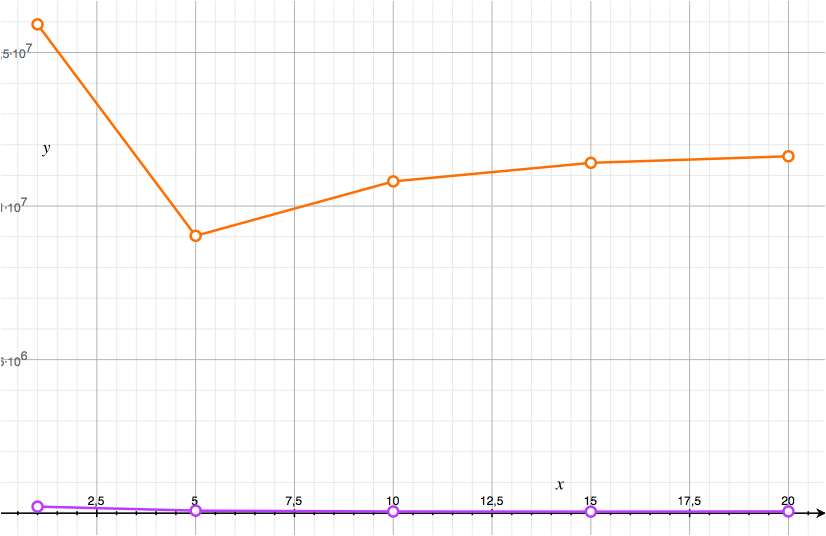
\includegraphics[width=0.8\textwidth]{graf2.jpg}
    \label{fig:latency}
    \caption{Graph showing local vs remote latency in our tests}
\end{figure}



\section{Reliability of the metrics}
As a general metric the latency and throughput are great, but it would also be interesting to do some research in terms of profiling the code and hardware, i.e. if we have to use a lot of resources to swap memory in and out in an implementation on a certain hardware setup it would possibly influence the other metrics or the overall stability of the system. Accordingly if we were just hogging memory rather than swapping this issue might not be visible through the latency and throughput metrics, thus it would be an interesting metric to take into account in the real world often too.

